\documentclass[11pt]{article}
\usepackage{enumerate}
\usepackage{fullpage}
\usepackage{fancyhdr}
\usepackage{amsmath, amsfonts, amsthm, amssymb}
\usepackage{color}
\usepackage[]{graphicx}
\setlength{\parindent}{0pt}
\setlength{\parskip}{5pt plus 1pt}
\pagestyle{empty}

\def\indented#1{\list{}{}\item[]}
\let\indented=\endlist

\newcounter{questionCounter}
\newcounter{partCounter}[questionCounter]
\newenvironment{question}[2][\arabic{questionCounter}]{%
    \setcounter{partCounter}{0}%
    \vspace{.25in} \hrule \vspace{0.5em}%
        \noindent{\bf #2}%
    \vspace{0.8em} \hrule \vspace{.10in}%
    \addtocounter{questionCounter}{1}%
}{}
\renewenvironment{part}[1][\alph{partCounter}]{%
    \addtocounter{partCounter}{1}%
    \vspace{.10in}%
    \begin{indented}%
       {\bf (#1)} %
}{\end{indented}}

%%%%%%%%%%%%%%%%%%%%%%%HEADER%%%%%%%%%%%%%%%%%%%%%%%%%%%%%%
\newcommand{\myname}{Shashank Singh}
\newcommand{\myandrew}{sss1@andrew.cmu.edu}
\newcommand{\myclass}{15-423 Digital Signal Processing for CS}
\newcommand{\duedate}{Tuesday, May 14, 2013}
%%%%%%%%%%%%%%%%%%%%%%%%%%%%%%%%%%%%%%%%%%%%%%%%%%%%%%%%%%%

%%%%%%%%%%%%%%%%%%%%CONTENT MACROS%%%%%%%%%%%%%%%%%%%%%%%%%
\renewcommand{\qed}{\quad $\blacksquare$}
\newcommand{\mqed}{\quad \blacksquare}
\newcommand{\inv}{^{-1}}
\newcommand{\N}{\mathbb{N}} % natural numbers
\newcommand{\Z}{\mathbb{Z}} % integers
\newcommand{\Zt}{\mathcal{Z}} % Z-transform
\newcommand{\Ft}{\mathcal{F}} % Fourier transform
\newcommand{\Q}{\mathbb{Q}} % rational numbers
\newcommand{\R}{\mathbb{R}} % real numbers
\newcommand{\C}{\mathbb{C}} % real numbers
\newcommand{\sminus}{\backslash} % asymmetric set difference
\newcommand{\I}{\mathcal{I}}
\newcommand{\E}{\mathcal{E}v} % even part of a signal
\renewcommand{\O}{\mathcal{O}d} % odd part of a signal
%%%%%%%%%%%%%%%%%%%%%%%%%%%%%%%%%%%%%%%%%%%%%%%%%%%%%%%%%%%

\begin{document}
\thispagestyle{plain}

{\Large Final Exam} \\
\myclass \\
Name: \myname \\
Email: \myandrew \\
Due: \duedate

\section{Signals}
\begin{enumerate}[1.]
\item See Figure~\ref{fig:1.1.1-4} for graphs.
\begin{figure}[h]
\begin{center}
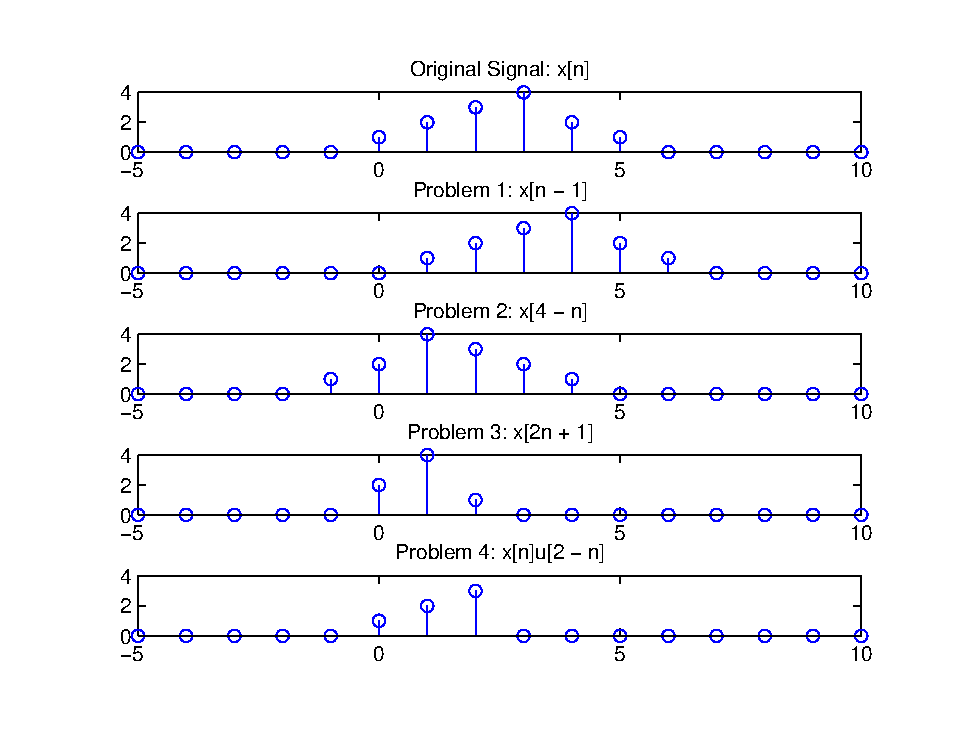
\includegraphics[width=0.8\textwidth]{1.1.1-4.eps}
\end{center}
\vspace{-0.6in}
\caption{A signal $x[n]$ and some of its variants.}
\label{fig:1.1.1-4}
\end{figure}

\item
\begin{enumerate}[1.]
\item
$x[n]$ is not periodic.

\item
$x[n]$ is periodic with period $T = 7$, since
$\exp\left(j\frac{8\pi t}{7} + \phi \right)$ has period $7/4$.

\item
$x(t)$ is periodic with period $T = \frac{2\pi}{7}$.

\item
$x(t)$ is not periodic.

\end{enumerate}

\end{enumerate}

\newpage
\section{Systems}
\begin{enumerate}[1.]
\item The properties of each signal are given in the table below:
\vspace{-0.2in}
\begin{center}
\newcommand\sysfive{
\left\{
    \begin{array}{cl}
        x[n]    &   n > 0   \\
        0       &   n = 0   \\
        -x[n]   &   n < 0
    \end{array}
\right.
}
\begin{tabular}{|c|c|c|c|c|c|c|}
\hline
Problem     & System                        & Memoryless   & Shift-Invariant
    & Linear    & Causal    & Stable    \\
\hline
1           & $y[n] = x[n]x[n - 1]$         & No           & Yes
    & No        & Yes       & Yes       \\
\hline
2           & $y[n] = nx[n]$                & Yes          & No
    & Yes       & Yes       & No        \\
\hline
3           & $y[n] = x[2n] - 0.1y[n - 1]$  & No           & No
    & Yes       & No        & Yes       \\
\hline
4           & $y(t) = \sin(\omega t)x(t)$   & Yes           & No
    & Yes       & Yes       & Yes       \\
\hline
5           & $y(t) = \sysfive$             & Yes           & No
    & Yes       & Yes       & Yes       \\
\hline
\end{tabular}
\end{center}

%TODO
\item
\begin{enumerate}[1.]
\item
By bilinearity and associativity of the convolution, the entire system response
is to an input $x$ is
\[(x * h_1 + x * h_2) * h_3 = x * ((h_1 + h_2) * h_3).\]
It follows from bilinearity and shift-invariance of the convolution that the
entire system is linear and shift-invariant. \qed

\item
The output of the system is $x * ((h_1 + h_2) * h_3)$. The following MATLAB
computation gives the result displayed in Figure~\ref{fig:2.2.2}:
\begin{verbatim}
>> h1 = [zeros(1,4) 0:4 zeros(1,7)];  
>> h2 = [zeros(1,9) 3:-1:0 zeros(1,3)];
>> h3 = [zeros(1,4) ones(1,7) zeros(1,5)];
>> x = h3;
>> y = conv(x,conv((h1 + h2),h3));
\end{verbatim}
\vspace{-0.2in}
\begin{figure}[h]
\begin{center}
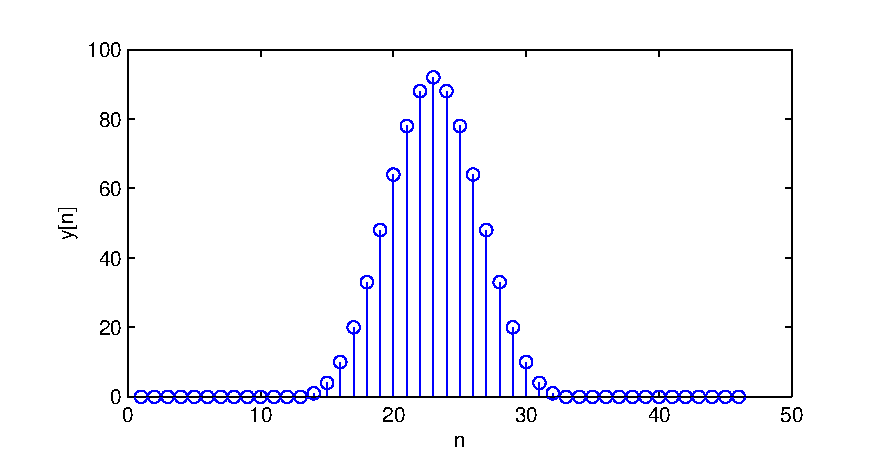
\includegraphics[width=0.8\textwidth]{2.2.2.eps}
\end{center}
\vspace{-0.2in}
\caption{The response $y$ of the composite system $h$ to the input $x$.}
\label{fig:2.2.2}
\end{figure}

\end{enumerate}
\end{enumerate}

%TODO
\section{Transforms}
\subsection{Fourier Transforms}
\begin{enumerate}
%TODO
\item 
\begin{itemize}
%TODO
\item The following MATLAB code computes the discrete Fourier series
coefficients:
\begin{verbatim}
>> for k = 0:11
     for n=0:11
       a(k+1,n+1) = (sin(2*pi*n/3)*cos(pi*n/2))*exp(-i*k*2*pi*n/12);
     end
   end
>> sum(a,2)/12

ans =

   0.0000          
   0.0000 - 0.2500i
  -0.0000 + 0.0000i
   0.0000 + 0.0000i
   0.0000 + 0.0000i
  -0.0000 + 0.2500i
   0.0000 - 0.0000i
  -0.0000 - 0.2500i
  -0.0000 - 0.0000i
   0.0000 - 0.0000i
   0.0000 - 0.0000i
  -0.0000 + 0.2500i
\end{verbatim}


\item The following MATLAB code computes the discrete Fourier series
coefficients:
\begin{verbatim}
>> for k = 0:5
     for n=-2:3
       a(k+1,n+3) = ((1/2)^n)*exp(-i*k*2*pi*n/6);
     end
   end
>> sum(a,2)/6

ans =

   1.3125          
   0.0000 + 0.7578i
  -0.3750 - 0.3248i
   0.4375 - 0.0000i
  -0.3750 + 0.3248i
   0.0000 - 0.7578i
\end{verbatim}

\newpage
\item
\begin{verbatim}
>> for k = 0:7
     for n=0:7
       a(k+1,n+1) = (x(n+1))*exp(-i*k*2*pi*n/8);                       
     end
   end
>> sum(a,2)/8 

ans =

   0.5335          
   0.0000 - 0.1875i
   0.1083 - 0.2500i
   0.0000 + 0.0000i
   0.3583 + 0.0000i
  -0.0000 + 0.1875i
  -0.2165 + 0.2500i
   0.0000 - 0.1875i
  -0.0000 - 0.0000i
   0.0000 - 0.0000i
   0.0000 - 0.0000i
  -0.0000 + 0.3750i
\end{verbatim}

\end{itemize}

%TODO
\item I chose not to do this problem.

%TODO
\item 
\begin{itemize}
%TODO
\item I didn't have time to finish this problem.

%TODO
\item I didn't have time to finish this problem.

%TODO
\item Letting
\[I(t) := \sum_{k \in \Z} \delta(t - k)\]
denote a unit impulse train, note that $x(t) = I(t) + I(t/2)$. Recalling that
$\Ft \{ I(t) \} = 2\pi I \left( \frac{\omega}{2\pi} \right)$, by linearity and
the time-scaling property of Fourier Transforms,
\[\mbox{\fbox{$\displaystyle \Ft \{ x(t) \}
    = 2\pi \left( I \left( \frac{\omega}{2\pi} \right)
    + 2 I \left( \frac{\omega}{\pi} \right) \right)$}}
.\]
\end{itemize}

%TODO
\item Writing $x$ and $y^*$ as Inverse Fourier Transforms of Fourier Transforms
and recognizing that
\[\delta(\omega) = \frac{1}{2\pi} \int_{-\infty}^\infty e^{i\omega t} \, dt,
    \quad \forall \omega \in \R,\]
gives
\begin{align*}
\int_{-\infty}^\infty x(t)y^*(t) \, dt
 & = \int_{-\infty}^\infty
    \left( \frac{1}{2\pi} \int_{-\infty}^\infty X(\omega_1)e^{i\omega_1 t} \, d\omega_1 \right)
    \left( \frac{1}{2\pi} \int_{-\infty}^\infty Y^*(\omega_2)e^{-i\omega_2 t} \, d\omega_2 \right)
        \, dt   \\
 & = \frac{1}{2\pi} \int_{-\infty}^\infty \int_{-\infty}^\infty X(\omega_1)Y^*(\omega_2)
     \frac{1}{2\pi} \int_{-\infty}^\infty e^{i(\omega_1 - \omega_2) t} \, dt
        \, d\omega_1 \, d\omega_1   \\
 & = \frac{1}{2\pi} \int_{-\infty}^\infty X(\omega_1) \int_{-\infty}^\infty Y^*(\omega_2)
     \delta(\omega_1 - \omega_2)    \, d\omega_2 \, d\omega_1   \\
 & = \frac{1}{2\pi} \int_{-\infty}^\infty X(\omega_1)Y^*(\omega_1)
     \, d\omega_2
\end{align*}
since convolution with a $\delta(x)$ function results in translation by $x$.
\qed
\end{enumerate}
\subsection{Z-Transforms}
\begin{enumerate}
%TODO
\item
\begin{itemize}
%TODO
\item I didn't have time to finish this problem.

\item 
\[\Zt\{ x[n] \}
    = \sum_{n = -\infty}^\infty x[n] z^{-n}
    = \sum_{n = -\infty}^{-1} (z/2)^{-n}
    + \sum_{n = 0}^\infty (2z)^{-n}
    = \frac{1}{1 - z/2} + \frac{1}{1 - (2z)\inv}.
\]

\item
\[\Zt\{ x[n] \}
    = \sum_{n = -\infty}^\infty x[n] z^{-n}
    = \sum_{n = 0}^9 z^{-n}
    = \frac{1 - z^{-10}}{1 - z\inv}.
\]
\end{itemize}

%TODO
\item 
\begin{itemize}
%TODO
\item I didn't have time to finish this problem.

\item The poles are $z = 2$ and $z = 1/2$. The ROC is $\{1/2 < |z| < 2\}$, and
hence the sequence has a Fourier transform.

\item The only pole is at the origin.
The ROC is the entire plane, and hence the sequence has a Fourier transform.
\end{itemize}

%TODO
\item I chose not to do this problem.

%TODO
\item I didn't have time to finish this problem.

\end{enumerate}

%TODO
\section{Filters}
\begin{enumerate}[I.]
%TODO
\item

%TODO
\item

\end{enumerate}
\end{document}
